\chapter{Cloud storage}
After going through CPU and network virtualization, it's time to talk about
proper ways of handling storaged data. In the age of \emph{cloud computing}
there's a huge amount of data to store, access and secure, so novel approches
to system design are necessary. To achieve the goal of cloud computation,
effective data replication and appropriate storage management strategies are
critical.

In the past, storage systems were designed according to a
\emph{performance-at-any-cost} philosophy, but now there's been a shift towards
\emph{reliability-at-the-lowest-possible-cost}. For example, data replication
allows concurrent access to data from multiple processors and decreases the
chances of data loss, but maintaining consistency among multiple copies of data
records increases complexity of the management software and could negatively
affect the storage system performance as a whole if data is frequently updated.

So, in this chapter we're going to explain some modern strategies adopted
to manage cloud storage while also respecting performance and realibility
requirements.

\section{Preliminary definitions}
Before proceding, we need to fix some concepts.

\begin{definition}[Storage model]
    A storage model describes the layout of a data structure in a physical storage.
\end{definition}
\begin{definition}[Data model]
    A data model captures the most important logical aspects of a data structure
    in a database
\end{definition}

\begin{definition}[Read-write coherence]
    The result of reading of a memory cell, should be the same as the most recent
    writing done on that cell.
\end{definition}
\begin{definition}[Before-or-after atomicity]
    The result of every read or write operation is the same as if that
    operation has been performed completely before or after another read or
    write operation.
\end{definition}

\noindent
\emph{Read-write coherence} and \emph{Before-or-after atomicity} are two highly
desirable properties of any \emph{storage model}.

\subsection{Types of storage}
There are three main types of storage:
\begin{enumerate}
    \item \emph{Block storage}: data is managed as blocks within sectors and
    tracks. Can be used when storage has access to raw and unformatted hardware
    and is useful when both speed and efficiency are important;
    \item \emph{File storage}: data is organized as structured files which are
    managed through a file system. However, this doesn't work very well with
    large amounts of data or when there's high-demand for a particular piece
    of data;
    \item \emph{Object storage}: data is managed as objects. Typically, each
    object has a gloabal unique identifier and holds both the data itself and
    some metadata. It's possible to access whole objects or blobs of data, but
    random accesses to data within an object is more difficult;
\end{enumerate}

\noindent
\emph{Block storage} is often used for database because it's the ideal way of
storing relational information. On the other hand, \emph{Object storage} isn't
suitable for databases, but is preferable to store content that can grow without
bounds, for example, backups and archives. Finally, the \emph{File storage} model
can be easily used to create \emph{distributed file system} via network protocols.

Examples of \emph{Block storage}, \emph{File storage} and \emph{Object storage}
are, respectivelly, \emph{Cinder}, \emph{Google file system} and OpenStack Swift.

\section{Block storage}
We'll give a quick look to this model by scratching the surface of \emph{OpenStack
Cinder}. \emph{OpenStack Cinder} implements services and libraries to provide
on-demand, self-service access to block storage resources. It provides API to
interact with storage backends which is also exposed to the cloud. End users can
manage their storage without knowing how it's organized and for both physical and
virtual environments.

\begin{figure}[h!]
    \centering
    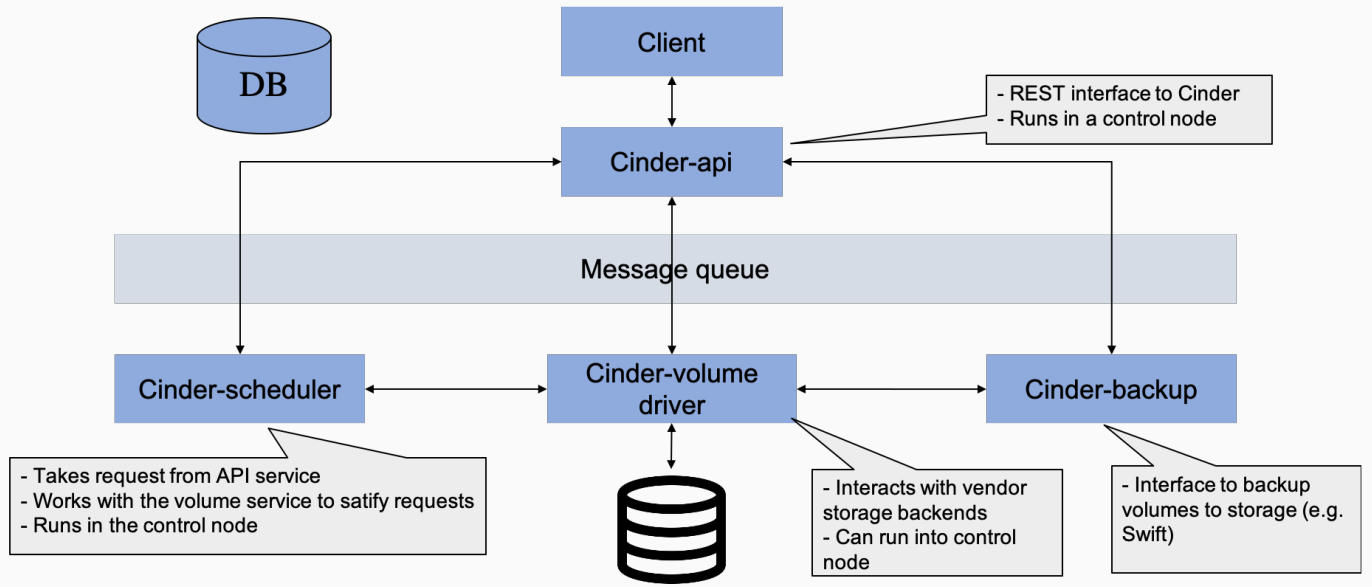
\includegraphics[width=0.7\textwidth]{images/block-model-cinder.png}
    \caption{\emph{OpenStack Cinder basic architecture}}
\end{figure}

\noindent
\emph{Cinder} APIs allow users to create and delete volumes and snaphots (for
backup pourposes). Attach or detach volumes for the available storage, clone and
extend them, and so on.

\section{Distributed file system}
Again, we'll start by giving some definitions.

\begin{definition}[File]
    A file is a linear array of cells stored on a persistent storage device. It
    is seen by application as a collection of logical records, and it's stored
    on a physical device as a set of physical records, or blocks, of size
    dictated by the physical media.
\end{definition}
\begin{definition}[File pointer]
    A file pointer is a cell used as starting point for a read or write operation.
\end{definition}

\noindent
A file has a logical organisation that reflects the \emph{data model} from the
perspective of the application, and a physical orgnisation that reflects the
\emph{storage model} and describes the manner the file is stored on a given
storage media.

\begin{definition}[File system]
    A file system is a collection of directories and each directory provides
    information about a set of files. A file system controls how data is stored
    and retrieved.
\end{definition}

\subsection{Unix File System}
The \emph{Unix File System} (\emph{UFS}) has both a layered and hierarchical
design. The first allows it to separate the physical file structure from the
logical one, and this becomes useful when dealing with files stored both locally
and remotely. The hierarchical design, on the other hand, allows grouping of
files in directories, supports multiple levels of directories and collections of
directories and files; thus, supporting a good degree of scalability.

The metadata that \emph{UFS} uses includes file owner, access rights, creation
time, time of the last modification, file size, the structure of the file and
the persistent storage device cells where data is stored. All of these are
memorized in a structure called \emph{inode}. Each \emph{inode} holds information
about individual files and directories and is kept on persistent media together
with the actual data.

\bigskip\noindent
Going back to \emph{UFS} layering, there are two layers:
\begin{itemize}
    \item \emph{Lower layer}: is about the physical organisation and is furderly
    separated into three sub-layers:
    \begin{itemize}
        \item \emph{Block layer}: responsible for locating individual blocks on
        the physical device;
        \item \emph{File layer}: reflects the organisation of blocks into files;
        \item \emph{Inode layer}: provides metadata for files and directories;
    \end{itemize}
    \item \emph{Upper layer}: is about the logical orgnisation;
\end{itemize}

\newpage
\begin{figure}[ht!]
    \centering
    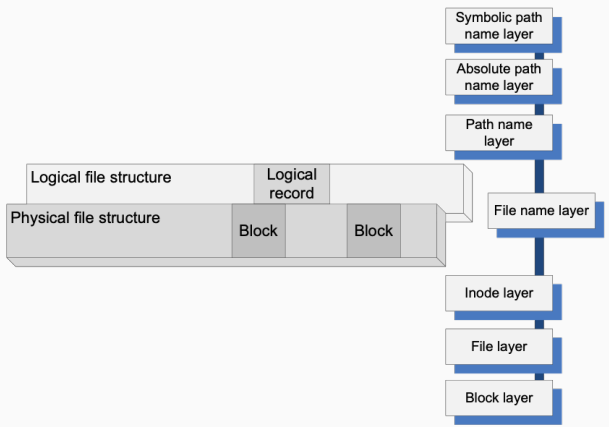
\includegraphics[width=0.6\textwidth]{images/ufs-layering.png}
    \caption{\emph{UFS} layering}
\end{figure}

\subsection{Network File System}
The \emph{Network File System} (\emph{NFS}) is designed to provide the same
semantics as the \emph{UFS} to ensure compatiblity with existing applications.
\emph{NFS} is based on the client-server paradigm and, in particular, clients
runs on the local host and interact with the server via remote procedure calls.

Each remote file is identified by a 32-bit file handler rather than a file
descriptor like in \emph{UFS}. A file handler is obtained combining a file
system identication, an \emph{inode} number and a generation number.

\begin{figure}[h!]
    \centering
    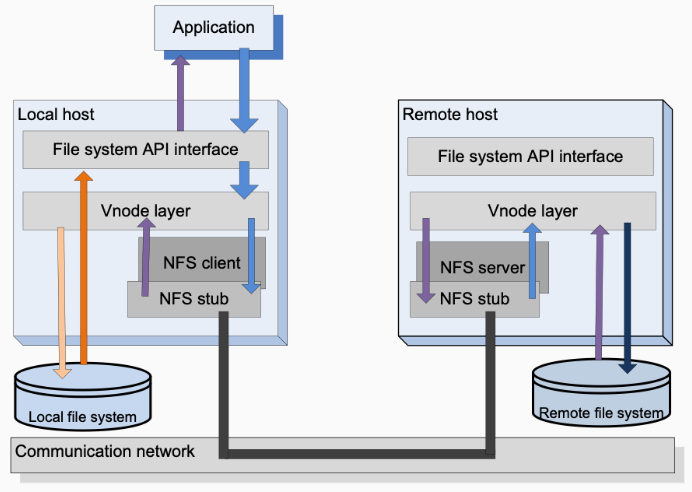
\includegraphics[width=0.6\textwidth]{images/nfs-design.png}
    \caption{\emph{NFS} design}
\end{figure}

\noindent
As the image shows, instead of an \emph{inode layer} the \emph{NFS} has a
\emph{vnode layer} which implements file operations in a uniform manner,
regardless of whether the file is local or remote. Also, an operation targeting
a local file is directed to the local file system without involving the \emph{NFS}.

When a client interacts with the server, the client-side \emph{NFS} packages the
relevant information about target, then sends those packaged information to the
server-side \emph{NFS}. The latter then passes the received information to the
\emph{vnode layer} of the remote host which finally directs it to the remote
file system.

\newpage
\begin{table}[ht!]
    \centering
    \begin{tabular}{|l|l|c|l|p{0.5\textwidth}|}
        \hline
        \textbf{API} & \textbf{Description} && \textbf{API} & \textbf{Description}\\
        \hline
        \texttt{fd} & File descriptor && \texttt{dfh} & The directory in which the file
        handle can be found\\
        \hline
        \texttt{fh} & File handle && \texttt{count} & Number of bytes to be transferred\\
        \hline
        \texttt{fname} & File name && \texttt{buf} & Buffer used to transfer data\\
        \hline
        \texttt{dname} & Directory name && \texttt{device} & The device in which the
        file system is located\\
        \hline
    \end{tabular}
    \caption{\emph{NFS} APIs}
\end{table}

\begin{figure}[h!]
    \centering
    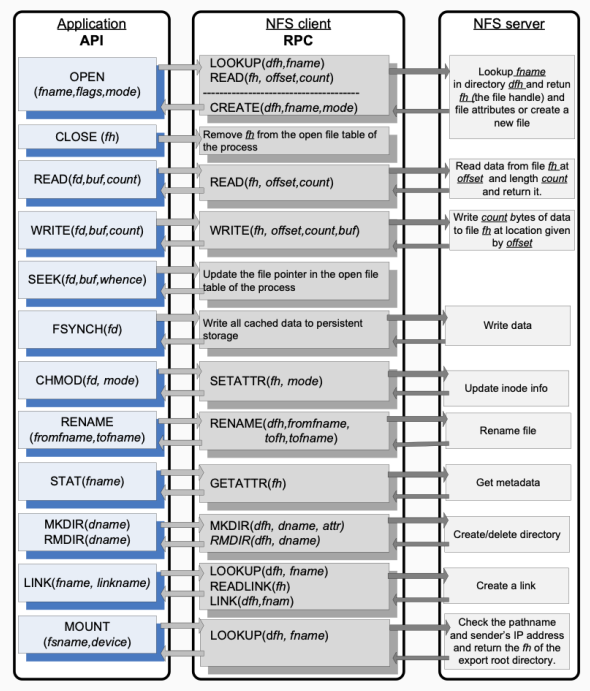
\includegraphics[width=0.6\textwidth]{images/nfs-remote-calls.png}
    \caption{\emph{UFS} APIs and corresponding \emph{NFS} remote procedure calls}
\end{figure}

\paragraph{Common design choices for distributed file system}
The vast majority of distributed file systems has been implemented in similar
ways. That's not so surprising if we think that they all need to solve the same
problems and that the possible or best solutions to choose from are limited.

Tipically, every distributed file system is implemented in a way that once a file
is closed, the server will have the newest version of it on persisten storage.
Another concern is about what to do when writing on a file. The possible
solutions are two:
\begin{enumerate}
    \item \emph{Write-through}: block is written to the disk as soon as it is
    available on the cache. This approch increases reliability, but it takes more
    time to complete each write operation;
    \item \emph{Delay in write-back}: a block is first written to cache and
    writing on the disk is delayed for a time in the order of tens of seconds.
    This speeds up writings and avoids useless writing when data is discarded
    before the time to save it to the disk. However, data can be lost in case
    of system failures;
\end{enumerate}

\noindent
Finally, how should the system act when multiple clients tries to access the
same file at the same time? The possibilities are two:
\begin{enumerate}
    \item \emph{Sequential write-sharing}: a file cannot be opened simultaneously
    for reading and writing by several clients;
    \item \emph{Concurrent write-sharing}: multiple clients can modify the same
    file at the same time (in a concurrent way, of course);
\end{enumerate}

\subsection{General Parallel File System}
\emph{General Paralles File System} (\emph{GPFS}) is a distributed file
system developed by IBM that's designed for optimal performance of large
clusters. To do so, it allows parallel I/O, meaning that multiple I/O
operations can be executed concurrently.

\begin{figure}[h!]
    \centering
    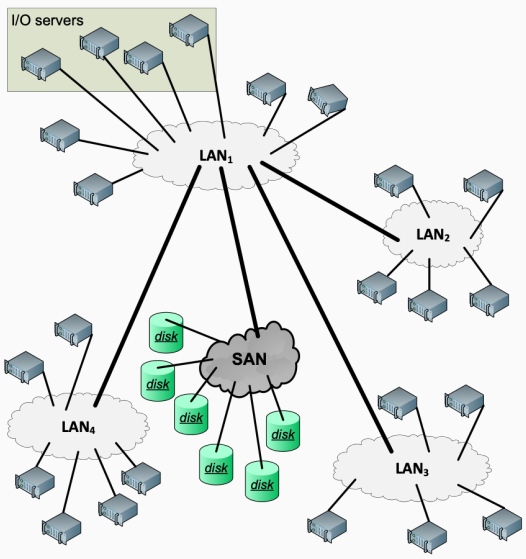
\includegraphics[width=0.6\textwidth]{images/gpfs-design.png}
    \caption{\emph{GPFS} architecture}
\end{figure}

\noindent
As the image shows, every disk is interconnected via a \emph{Storage Area Network}
(\emph{SAN}) and servers used to handle I/O are distributed in various LANs.

\emph{GPFS} is a realiable file system because it can recover from system
failures. To achive so, \emph{GPFS} records all metadata updates in a write-ahead
log file. Write-ahead means that updates are written to persisten storage only
after log records have been written. Every I/O node manages one log file for
each file system it mounts and any I/O node can initiate recovery on behalf of
a failed node.

Finally, \emph{GPFS} uses data striping to allow concurrent access and improve
performance. By using data striping, \emph{GPFS} segments logically sequential
data (e.g. files) so that consecutive segments are stored on different physical
storage devices. The problem with this approch is that a failed disk will affect
many more files. To reduce the impact of this and further improve fault tollerance,
\emph{GPFS} data files as well as metadata are replicated on two different
physical disks.

\subsection{Google File System}
\emph{Google File System} (\emph{GFS}) is another distributed file system,
developed by Google that uses thousands of storage devices built from inexpensive
commodity components to provide PBs of storage to a large user community
with various needs.

\begin{table}[h!]
    \centering
    \begin{tabular}{|p{0.47\textwidth}|p{0.47\textwidth}|}
        \hline
        \textbf{Design consideration} & \textbf{Design choice}\\
        \hline
        Vast majority of files range in size from a few GBs to hundreds of TBs &
        Files are segmented in large \emph{chunks}\\
        \hline
        Most common operation is to append to an existing file and random write
        operations to a file are extremely infrequent & Implement an atomic file
        append operation allowing multiple applications operating concurrently
        to append to the same file\\
        \hline
        Consistency model should be relaxed to simplify the system implementation
        but without placing an additional burden on the application developers &
        Ensure consistency by channeling critical file operations through a
        \emph{master}, a component of the cluster which controls the entire
        system\\
        \hline
    \end{tabular}
\end{table}

\noindent
Other considerations made are:
\begin{itemize}
    \item Scalability and reliability are critical features of the system, and
    they must be considered from the beginning, rather than at some stage of the
    design;
    \item Sequential read operations are the norm;
    \item Users process the data in bulk and are less concerned with the
    response time;
\end{itemize}
And other relevant design decisions are:
\begin{itemize}
    \item Cluster must be built around a high-bandwidth rather than a low-latency
    interconnection network, so control and data flows should be separated.
    High-bandwidth data flow should be scheduled by pipelining data transfer over
    TCP connections and finally, the network topology should be exploited by
    sending data to the closest node in the network;
    \item Caching at client side should be eliminated to reduce the overhead
    that's necessary for maintaining consistency among cached copies;
    \item Efficient checkpointing and fast recovery mechanisms should be
    supported as well as an efficient garbace colletor;
\end{itemize}

\paragraph{GFS chunks}
So, as we said, files are segmented into large \emph{chunks}. To be more precise
each \emph{chunk} is large exactly 64MB. This choice was motivated by the desire
to optimize performance for large files and to reduce the amount of metadata
maintained by the system. Also, large \emph{chunk} size increases the likelihood
that multiple operations will be directed to the same \emph{chunk}; thus it
reduces the number of requests to locate the \emph{chunk} and also allows
applications to maintain a persistent network connection with the server where
the \emph{chunk} is located.

A \emph{chunk} is then divided in 64KB blocks and each block holds a 32bit
checksum. Each \emph{chunk} is stored in a \emph{UFS} and is replicated on a
configurable amount of sites (default is 3 replicas). At the time of creation,
each \emph{chunk} is given a unique \emph{chunk} handle.

\paragraph{GFS architecture}
The following image shows the typical architecture of a \emph{GFS} implementation.
Each \emph{master} maintains state information about all system components and
control a number of \emph{chunk servers}. A \emph{chunk server} is basically a
Linux system and uses metadata provided by its \emph{master} to communicate
directly with the applications.

\begin{figure}[ht!]
    \centering
    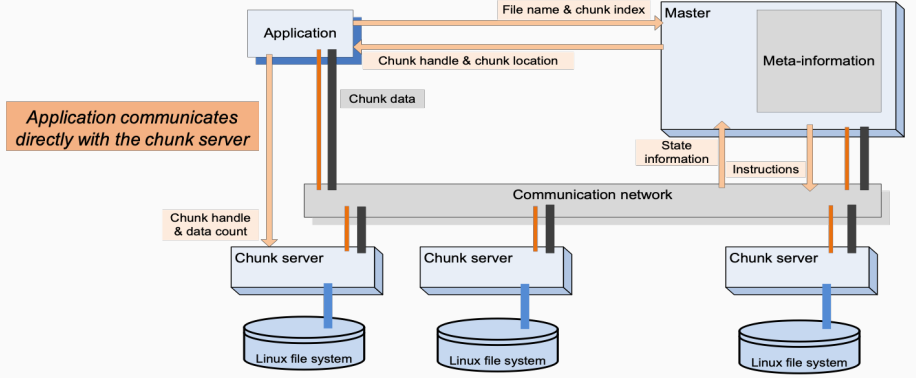
\includegraphics[width=0.6\textwidth]{images/gfs-architecture.png}
    \caption{\emph{GFS} architecture}
\end{figure}

\begin{note}
    Data and control flows have been graphically separated. Data paths
\end{note}

\paragraph{Steps for a write request}
Let's see the steps required to complete a generic write operation.
First, the client contacts the \emph{master} which replies with the location
of the primary and secondary replicas, that is, the \emph{master} replies with
the ID of the chuck servers that hold the required \emph{chunk}.

The \emph{master} will also assign a lease to the primary replica. That
server will have an exclusive permission to read, write and modify data of a
particulare \emph{chunk} without fear of another server changing it. When the
lease expires\footnotemark the \emph{master} must reassign the lease to another
server or the same server, depending on the needs of the system. This helps to
ensure data integrity and prevents data corruption.

\footnotetext{The lease time is usually aroung 60 seconds}

Then, the client sends data to all \emph{chunk servers} holding replicas, starting
from the closest to the furthest, and each one of them puts changes, aka
modifications, in a least recently used buffer and sends an acknowledgement back
to the client. Once the client has received all the expected acknowledgements,
it sends a write request to the primary replica.

That server applies modifications, then sends write requests to all secondaries,
which also apply modifications and send acknowledgements at the end. When the
primary replica has received all the expected acknowledgements, it sends a
final acknowledgement to the client.

\paragraph{Clarification about primary replicas and lease assignment}
The distinction between primary and secondary replicas exists just to decide
which one will communicate with the client. So, the choice might change over
time and is made by the \emph{master} based on what \emph{chunk server} is
closer to the client.

When the \emph{master} receives a request it first checks if any of the
\emph{chunk servers} already holds a lease. If any, that server will be the
primary replica even if it isn't the closest to the client.

\paragraph{Steps for a read request}
A read request is simpler than a write one. As before, the client sends a read
request to the \emph{master}, which replies with primary and secondary replicas
IDs. The client can then proced to contact the primary replica which responds
with the required data.

\section{Locks and consensus}